\section{ APP}

\begin{frame}[fragile]{CH10 XML的应用与挑战——SVG \& JSON}
\begin{figure}
    
\includegraphics[width=0.5\textwidth]{figure/app.png}
\end{figure}
\end{frame}

\begin{frame}[fragile]{本章学习目标}
\begin{easylist} \easyitem
& 了解SVG的特点
& 能够基于SVG进行简单的图形表示
& 了解d3.js的功能特点
& 掌握JSON的数据结构和类型
& 能够通过JavaScript解析JSON字符串

\end{easylist}
\end{frame}

\begin{frame}[fragile]{目录}
\begin{easylist} \easyitem
& 概述
& SVG
&& SVG的基本形状
&& SVG的样式设置
&& SVG的层与重叠
&& SVG的透明度
&& 基于SVG的d3.js图形绘制库
& JSON
&& JSON的数据结构
&& JSON的值类型
&& JSON与XML的对比
&& 利用JavaScript解析JSON
\end{easylist}
\end{frame}


\subsection{10.1 概述}

\begin{frame}[fragile]{10.1 概述}
\begin{easylist} \easyitem
& SVG
&& 可缩放矢量图形(Scalable Vector Graphics)
&& 1999年推出
& JSON
&& JavaScript Object Notation
&& 尤其适合作为数据传输格式
& SVG、JSON、XML是Web技术体系的重要组成部分
\end{easylist}
\end{frame}

\begin{frame}[fragile]{PNG与SVG文件缩放对比}
\begin{figure}
    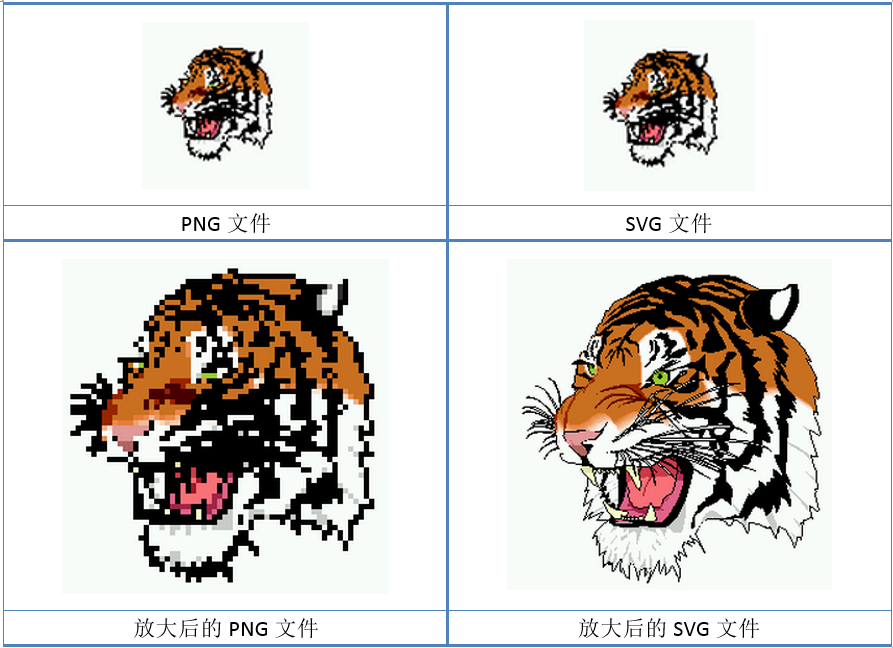
\includegraphics[width=0.85\textwidth]{figure/app-svg-vs-png.png}
\end{figure}
\end{frame}


\subsection{10.2 SVG}

\begin{frame}[fragile]{10.2 SVG}
\begin{easylist} \easyitem
& 通过XML定义线段、圆形、矩形等形状
\begin{lstlisting}[tabsize=8, basicstyle=\small\tt, language=XML]
<svg xmlns="http://www.w3.org/2000/svg" width="50" height="50">
    <circle cx="25" cy="25" r="22" fill="blue" stroke="gray" stroke-width="2"/>
</svg>
\end{lstlisting}
\end{easylist}
\end{frame}


\begin{frame}[fragile, allowframebreaks]{SVG示例}
\begin{lstlisting}[tabsize=8, basicstyle=\small\tt, language=HTML, caption="circle.html"]
<!DOCTYPE html>
<html>
    <head>
        <title>SVG Circle</title>
    </head>
    <body>
        <svg width="50" height="50">
            <circle cx="25" cy="25" r="22" fill="blue" stroke="gray" stroke-width="2"/>
        </svg>
    </body>
</html>
\end{lstlisting}

\begin{figure}
    
\includegraphics[width=0.2\textwidth]{figure/app-circle.png}
\end{figure}
\end{frame}


\begin{frame}[fragile]{Linux Imagte Viewer}
\begin{figure}
    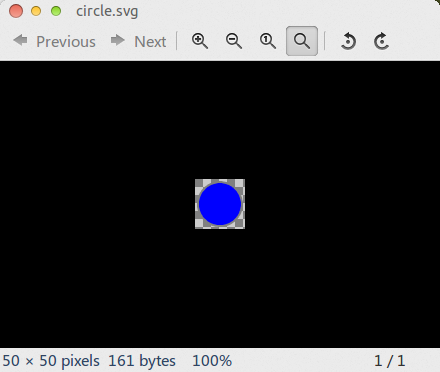
\includegraphics[width=0.4\textwidth]{figure/app-svg-viewer.png}
\end{figure}
\begin{figure}
    
\includegraphics[width=0.4\textwidth]{figure/app-svg-viewer2.png}
\end{figure}
\end{frame}


\subsubsection{10.2.1 SVG的基本形状}
\begin{frame}[fragile, allowframebreaks]{10.2.1 SVG的基本形状}
\begin{easylist} \easyitem
& 基本形状
&& 矩形:rect
&& 圆形:circlue
&& 椭圆:Ellipse
&& 线条:line
&& 文本:Text

& 坐标系
\begin{figure}
    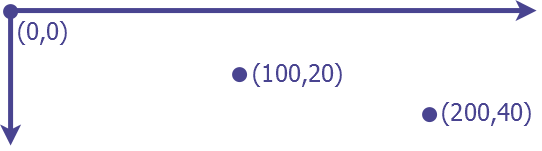
\includegraphics[width=0.9\textwidth]{figure/svg-coordinates.png}
\end{figure}
\end{easylist}
\end{frame}


\begin{frame}[fragile, allowframebreaks]{绘制矩形}
\begin{easylist} \easyitem
& 代码
\begin{lstlisting}[tabsize=8, basicstyle=\small\tt, language=XML, numbers=none]
<rect x="0" y="0" width="300" height="50"/>
\end{lstlisting}
& 效果
\begin{figure}
    
\includegraphics[width=0.5\textwidth]{figure/svg-rect.png}
\end{figure}

\newpage
& 代码
\begin{lstlisting}[tabsize=8, basicstyle=\small\tt, language=XML, numbers=none]
<rect x="0" y="0" width="300" height="50" rx="15" ry="15"/>
\end{lstlisting}
& 效果
\begin{figure}
    
\includegraphics[width=0.5\textwidth]{figure/svg-rect2.png}
\end{figure}
\end{easylist}
\end{frame}


\begin{frame}[fragile, allowframebreaks]{绘制椭圆}
\begin{easylist} \easyitem
& 代码
\begin{lstlisting}[tabsize=8, basicstyle=\small\tt, language=XML, numbers=none]
<ellipse cx="250" cy="25" rx="50" ry="25"/>
\end{lstlisting}
& 效果
\begin{figure}
    
\includegraphics[width=0.2\textwidth]{figure/svg-ellipse.png}
\end{figure}
\end{easylist}
\end{frame}


\begin{frame}[fragile, allowframebreaks]{绘制线条}
\begin{easylist} \easyitem
& 代码
\begin{lstlisting}[tabsize=8, basicstyle=\small\tt, language=XML, numbers=none]
<line x1="0" y1="0" x2="350" y2="50" stroke="black"/>
\end{lstlisting}
& 效果
\begin{figure}
    
\includegraphics[width=0.9\textwidth]{figure/svg-line.png}
\end{figure}
\end{easylist}
\end{frame}

\begin{frame}[fragile, allowframebreaks]{绘制文本}
\begin{easylist} \easyitem
& 代码
\begin{lstlisting}[tabsize=8, basicstyle=\small\tt, language=XML, numbers=none]
<text x="250" y="25" font-family="华文隶书" font-size="30" fill="navy">可缩放矢量图形</text>
\end{lstlisting}
& 效果
\begin{figure}
    
\includegraphics[width=0.5\textwidth]{figure/svg-text.png}
\end{figure}
\end{easylist}
\end{frame}



\subsubsection{10.2.2 SVG的样式设置}
\begin{frame}[fragile]{10.2.2 SVG的样式设置}
\begin{easylist} \easyitem
& 默认样式为黑色填充、无stroke
& fill
&& 填充色,取值为有效的CSS颜色值,如颜色名称red、blue,或者RGB、RGBA值。
& stroke
&& 线条的颜色值
& stroke-width
&& 数值,通常采用像素单位
& opacity
&& 透明度,介于0.0到1.0之间的数值,0.0表示完全透明,1.0表示完全不透明
& font-family、font-size
&& 应用于文本
\end{easylist}
\end{frame}


\begin{frame}[fragile]{样式关联方式}
\begin{easylist} \easyitem
& 内联方式
\begin{lstlisting}[tabsize=8, basicstyle=\small\tt, language=XML, numbers=none]
<circle cx="50" cy="50" r="30" fill="yellow" stroke="orange" stroke-width="10"/>
\end{lstlisting}
& CSS样式属性关联方式
\begin{lstlisting}[tabsize=8, basicstyle=\small\tt, language=XML, numbers=none]
<circle cx="50" cy="50" r="30" class="pumpkin"/>
\end{lstlisting}
&& 需要设置pumpkin样式
& 效果
\begin{figure}
    
\includegraphics[width=0.1\textwidth]{figure/svg-pumpkin.png}
\end{figure}
\end{easylist}
\end{frame}


\begin{frame}[fragile, allowframebreaks]{示例网页}
\begin{lstlisting}[tabsize=8, basicstyle=\small\tt, language=HTML]
<!DOCTYPE html>
<html>
    <head>
        <title>SVG Style</title>
        <style>
            .pumpkin {
                fill: yellow;
                stroke: orange;
                stroke-width: 10;
            }
        </style>
    </head>
    <body>
        <svg width="500px" height="200px">
            <circle cx="50" cy="50" r="30" class="pumpkin"/>
        </svg>
    </body>
</html>
\end{lstlisting}
\end{frame}


\subsubsection{10.2.3 SVG的层与重叠}
\begin{frame}[fragile]{10.2.3 SVG的层与重叠}
\begin{easylist} \easyitem
& 根据绘制的先后顺序予以覆盖
\begin{lstlisting}[tabsize=8, basicstyle=\small\tt, language=XML]
<rect x="0" y="0" width="50" height="50" fill="red"/>
<rect x="25" y="15" width="50" height="50" fill="green"/>
<rect x="50" y="30" width="50" height="50" fill="blue"/>
<rect x="75" y="45" width="50" height="50" fill="gray"/>
<rect x="100" y="60" width="50" height="50" fill="navy"/>
\end{lstlisting}

\begin{figure}
    
\includegraphics[width=0.4\textwidth]{figure/svg-overlapping.png}
\end{figure}
\end{easylist}
\end{frame}


\subsubsection{10.2.4 SVG的透明度}
\begin{frame}[fragile]{10.2.4 SVG的透明度}
\begin{easylist} \easyitem
& 使用带alpha的RGB颜色函数rgba()
& 设置opacity属性值。
\end{easylist}
\end{frame}


\begin{frame}[fragile, allowframebreaks]{rgba()}
\begin{easylist} \easyitem
& 代码:
\begin{lstlisting}[tabsize=8, basicstyle=\small\tt, language=XML]
<circle cx="50" cy="50" r="40" fill="rgba(0, 150, 150, 1.0)"/>
<circle cx="100" cy="50" r="40" fill="rgba(0, 0, 255, 0.75)"/>
<circle cx="150" cy="50" r="40" fill="rgba(0, 255, 0, 0.5)"/>
<circle cx="200" cy="50" r="40" fill="rgba(255, 255, 0, 0.6)"/>
<circle cx="250" cy="50" r="40" fill="rgba(255, 0, 0, 0.3)"/>
\end{lstlisting}
& 显示效果:
\begin{figure}
    
\includegraphics[width=0.4\textwidth]{figure/svg-rgba.png}
\end{figure}

\newpage
& 代码:
\begin{lstlisting}[tabsize=8, basicstyle=\small\tt, language=XML]
<circle cx="50" cy="50" r="40" fill="rgba(0, 150, 150, 1.0)" 
        stroke="rgba(0, 255, 0, 0.25)" stroke-width="10"/>
<circle cx="100" cy="50" r="40" fill="rgba(0, 0, 255, 0.75)" 
        stroke="rgba(0, 0, 255, 0.25)" stroke-width="10"/>
<circle cx="150" cy="50" r="40" fill="rgba(0, 255, 0, 0.5)" 
        stroke="rgba(0, 0, 255, 0.25)" stroke-width="10"/>
<circle cx="200" cy="50" r="40" fill="rgba(255, 255, 0, 0.6)" 
        stroke="rgba(255, 0, 0, 0.25)" stroke-width="10"/>
<circle cx="250" cy="50" r="40" fill="rgba(255, 0, 0, 0.3)" 
        stroke="rgba(55, 255, 0, 0.25)" stroke-width="10"/>
\end{lstlisting}
& 显示效果:
\begin{figure}
    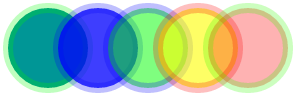
\includegraphics[width=0.4\textwidth]{figure/svg-rgba2.png}
\end{figure}
\end{easylist}
\end{frame}


\begin{frame}[fragile, allowframebreaks]{opacity}
\begin{easylist} \easyitem
& opacity设置为1.0表示完全不透明,为默认值
\begin{lstlisting}[tabsize=8, basicstyle=\small\tt, language=XML]
<circle cx="50" cy="50" r="40" fill="green" stroke="orange" stroke-width="10" opacity="1.0"/>
<circle cx="120" cy="50" r="40" fill="yellow" stroke="red" stroke-width="10"/>
<circle cx="190" cy="50" r="40" fill="orange" stroke="blue" stroke-width="10"/>
\end{lstlisting}
& 显示效果:
\begin{figure}
    
\includegraphics[width=0.4\textwidth]{figure/svg-opacity.png}
\end{figure}

\newpage
& 代码:
\begin{lstlisting}[tabsize=8, basicstyle=\small\tt, language=XML]
<circle cx="50" cy="50" r="40" fill="green" stroke="orange" stroke-width="10" opacity="0.5"/>
<circle cx="120" cy="50" r="40" fill="yellow" stroke="red" stroke-width="10" opacity="0.3"/>
<circle cx="190" cy="50" r="40" fill="orange" stroke="blue" stroke-width="10" opacity="0.1"/>
\end{lstlisting}
& 显示效果:
\begin{figure}
    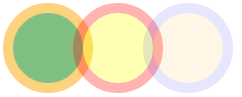
\includegraphics[width=0.4\textwidth]{figure/svg-opacity2.png}
\end{figure}
\end{easylist}
\end{frame}


\begin{frame}[fragile, allowframebreaks]{同时设置rgba与opacity}
\begin{easylist} \easyitem
& 代码:
\begin{lstlisting}[tabsize=8, basicstyle=\small\tt, language=XML]
<circle cx="50" cy="50" r="40" fill="green" stroke="orange" stroke-width="10" opacity="0.5"/>
<circle cx="120" cy="50" r="40" fill="yellow" 
        stroke="rgba(255, 0, 0, 0.5)" stroke-width="10" opacity="0.3"/>
<circle cx="190" cy="50" r="40" fill="orange" stroke="blue" stroke-width="10" opacity="0.1"/>
\end{lstlisting}
& 显示效果:
\begin{figure}
    
\includegraphics[width=0.4\textwidth]{figure/svg-opacity3.png}
\end{figure}
\end{easylist}
\end{frame}



\subsubsection{10.2.5 d3.js}
\begin{frame}[fragile]{10.2.5 d3.js}
\begin{easylist} \easyitem
& d3
&& Data-Driven Documents的缩写
&& Data表示用户提供的数据
&& Documents代表可以被浏览器解析呈现的文档,
&& 支持SVG
\end{easylist}
\end{frame}

\begin{frame}[fragile, allowframebreaks]{效果图}
\begin{figure}
    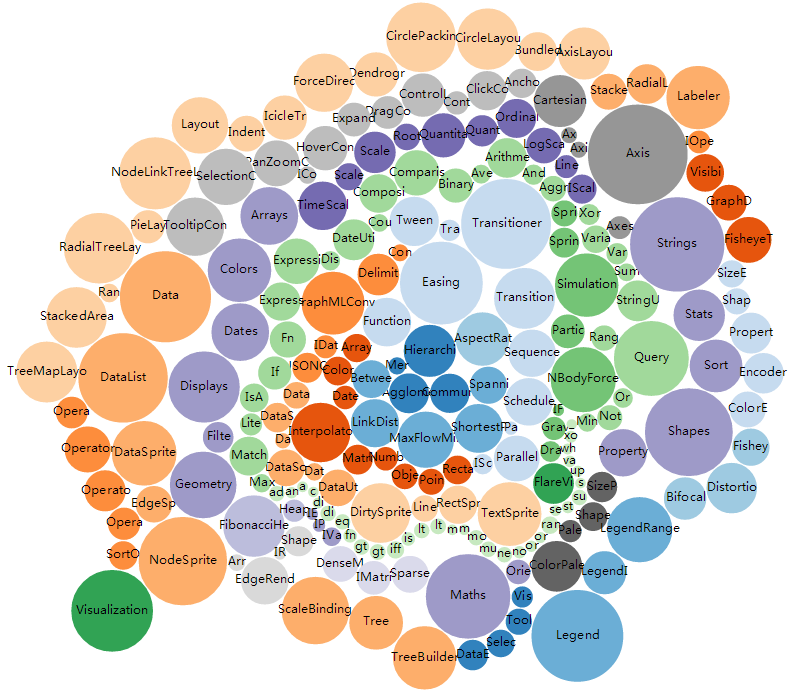
\includegraphics[width=0.5\textwidth]{figure/d3.demo1.png}
\end{figure}

\newpage
\begin{figure}
    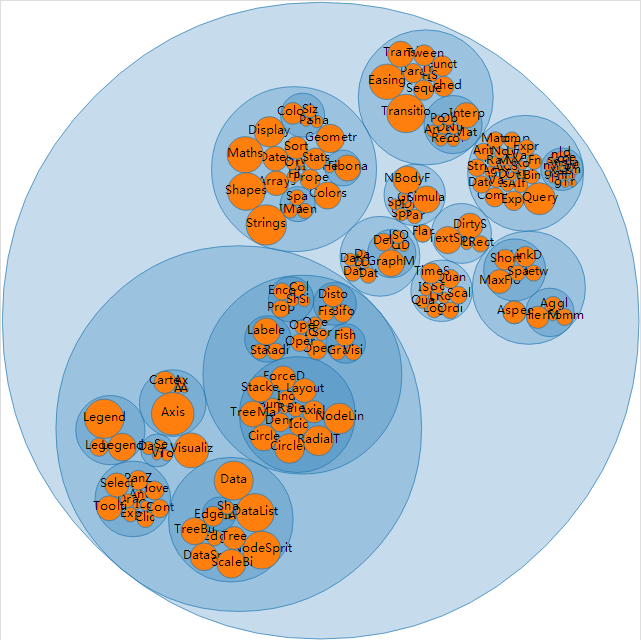
\includegraphics[width=0.5\textwidth]{figure/d3.demo2.png}
\end{figure}
\newpage
\begin{figure}
    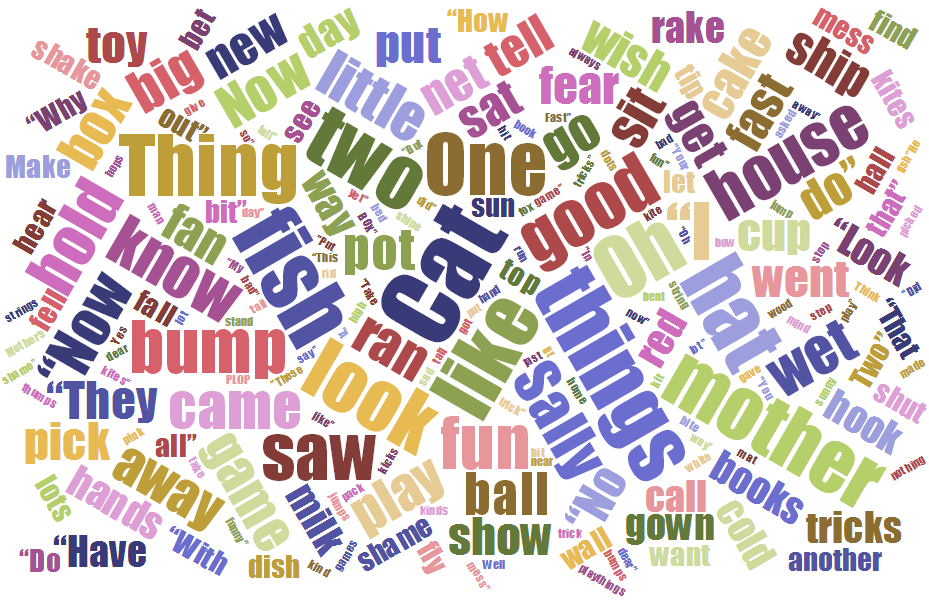
\includegraphics[width=0.5\textwidth]{figure/d3.demo3.png}
\end{figure}
\newpage
\begin{figure}
    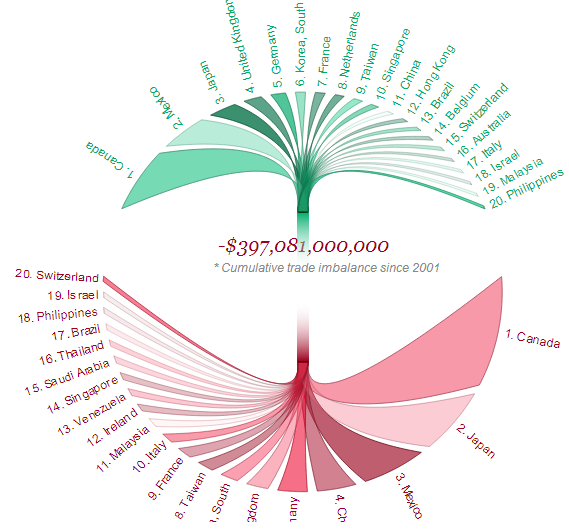
\includegraphics[width=0.5\textwidth]{figure/d3.demo4.png}
\end{figure}
\end{frame}


\begin{frame}[fragile]{如何引用d3.js进行测试}
\begin{easylist} \easyitem
& 下载最新版本的d3.js
& 在网页中引用d3.js
& 在Web Server中测试(可选)
\end{easylist}
\end{frame}


\begin{frame}[fragile, allowframebreaks]{基于d3.js绘制SVG图形}
\begin{easylist} \easyitem
& 创建svg元素,设置属性
\begin{lstlisting}[tabsize=8, basicstyle=\small\tt, language=JavaScript,numbers=none]
var svg = d3.select("body").append("svg");
svg.attr("width", 500);
svg.attr("height", 200);
\end{lstlisting}

& 采用链式语法改写
\begin{lstlisting}[tabsize=8, basicstyle=\small\tt, language=JavaScript,numbers=none]
var svg = d3.select("body") 
        .append("svg")
        .attr("width", 500)
        .attr("height", 200);
\end{lstlisting}

& 继续增加若干圆形
\begin{lstlisting}[tabsize=8, basicstyle=\small\tt, language=JavaScript,numbers=none]
var dataset = [ 20, 15, 10, 5, 10, 15, 20 ];
var circles = svg.selectAll("circle")
        .data(dataset)
        .enter()
        .append("circle");
\end{lstlisting}

& 继续指定图形的位置和大小
\begin{lstlisting}[tabsize=8, basicstyle=\small\tt, language=JavaScript,numbers=none]
circles.attr("cx", function(d, i) {
            return (i * 50) + 25;
          })
        .attr("cy", 50)
        .attr("r", function(d) {
            return d;
          });
\end{lstlisting}
&& 代码中d表示传入函数的绑定数据,i代表图形顺序编号,起始编号为0
& 显示效果
\begin{figure}
    
\includegraphics[width=0.5\textwidth]{figure/d3.circles.png}
\end{figure}
& 继续指定圆的样式
\begin{lstlisting}[tabsize=8, basicstyle=\small\tt, language=JavaScript,numbers=none]
.attr("fill", "orange")
.attr("stroke", "red")
.attr("stroke-width", function(d, i) {
    return d/3;
});
\end{lstlisting}
& 显示效果
\begin{figure}
    
\includegraphics[width=0.5\textwidth]{figure/d3.circles2.png}
\end{figure}
\end{easylist}
\end{frame}




\begin{frame}[fragile, allowframebreaks]{代码清单}
\begin{lstlisting}[tabsize=8, basicstyle=\small\tt, language=HTML]
<!DOCTYPE html>
<html>
    <head>
        <meta charset="utf-8" />
        <title>D3 Circles</title>
        <script type="text/javascript" src="d3/d3.v3.js"></script>
    </head>
    <body>
        <script type="text/javascript">
            var svg = d3.select("body")
                    .append("svg")
                    .attr("width", 500) 
                    .attr("height", 200); 
            var dataset = [20, 15, 10, 5, 10, 15, 20]; 
            var circles = svg.selectAll("circle")
                              .data(dataset) 
                              .enter()
                              .append("circle");

            circles.attr("cx", function(d, i) {
                return (i * 50) + 25; 
            })
            .attr("cy", 50) 
            .attr("r", function(d) {
                return d; 
            })
            .attr("fill", "orange")
            .attr("stroke", "red")
            .attr("stroke-width", function(d, i) {
                return d/3; 
            });
        </script>
    </body>
</html>
\end{lstlisting}
\end{frame}



\subsection{10.3 JSON}

\begin{frame}[fragile]{10.3 数据传输的挑战者—JSON}
\begin{easylist} \easyitem
& JSON
&& JavaScript Object Notation
&& 一种轻量级、基于文本、语言无关的数据交换格式
&& JavaScript(Standard ECMA-262)的一个子集
&& 重要贡献者:Douglas Crockford
&& 2006年7月——RFC 4627
\end{easylist}
\end{frame}


\subsubsection{10.3.1 JSON的数据结构}
\begin{frame}[fragile]{10.3.1 JSON的数据结构}
\begin{easylist} \easyitem
& 无序的键值对集合
\begin{lstlisting}[tabsize=8, basicstyle=\small\tt, language=JavaScript, numbers=none]
{ "a":1,"b":2,"c":3 }
\end{lstlisting}
& 值的有序列表
\begin{lstlisting}[tabsize=8, basicstyle=\small\tt, language=JavaScript, numbers=none]
[ 1, 2, 3, "hello world" ]
\end{lstlisting}
\end{easylist}
\end{frame}


\subsubsection{10.3.2 JSON的值类型}
\begin{frame}[fragile]{10.3.2 JSON的值类型}
\begin{easylist} \easyitem
& 符串类型
&& JSON字符串采用双引号包括所表示的字符内容,字符内容本身包含的双引号使用反斜线进行转义;
& 数值类型
& 对象类型
&& 键值对的无序集合;
& 数组类型
&& 值的有序列表;
& 布尔类型
&& true表示真、false表示假;
& 空类型null
\end{easylist}
\end{frame}

\begin{frame}[fragile, allowframebreaks]{JSON示例}
\begin{lstlisting}[tabsize=8, basicstyle=\small\tt, language=JavaScript, caption=contact.json]
{
    "name": "王某某",
    "age": 30,
    "spouse": {
        "name": "张某某",
        "age": 28
    },
    "addresses": [
        {
            "description": "工作住址",
            "street": "胜利大街9号",
            "city": "潍坊",
            "province": "山东"
        }
    ], 
    "phoneNumbers": [
        {
            "description": "办公电话",
            "number": "6666-7777"
        },
        {
            "description": "手机",
            "number": "1XX-1234-5678"
        }
    ]
}
\end{lstlisting}
\end{frame}


\subsubsection{10.3.3 JSON与XML的对比}
\begin{frame}[fragile]{10.3.3 JSON与XML的对比}
\begin{easylist} \easyitem
& XML比JSON更易于人工阅读
& XML是典型的标记语言,而JSON不是
& JSON格式简洁,文件的体积较小,有利于数据传输。
& JSON与JavaScript结合紧密,构造和解析都比较容易,而通过JavaScript解析XML,则需要借助于额外的库
\end{easylist}
\end{frame}


\begin{frame}[fragile, allowframebreaks]{contact.json对应的XML}
\begin{lstlisting}[tabsize=8, basicstyle=\small\tt, language=XML, caption=contact.xml]
<contact>
    <name>王某某</name>
    <age>30</age>
    <spouse>
        <name>张某某</name>
        <age>28</age>
    </spouse>
    <addresses>
        <address>
            <description>工作住址</description>
            <street>胜利大街9号</street>
            <city>潍坊</city>
            <province>山东</province>
        </address>
    </addresses>
    <phoneNumbers>
        <phoneNumber>
            <description>办公电话</description>
            <number>6666-7777</number>
        </phoneNumber>
        <phoneNumber>
            <description>手机</description>
            <number>1XX-1234-5678</number>
        </phoneNumber>
    </phoneNumbers>
</contact>
\end{lstlisting}
\end{frame}


\subsubsection{10.3.4 利用JavaScript解析JSON}
\begin{frame}[fragile]{10.3.4 利用JavaScript解析JSON}
\begin{easylist} \easyitem
& 浏览器内置的JSON.parse()
\begin{lstlisting}[tabsize=8, basicstyle=\small\tt, language=JavaScript, numbers=none]
JSON.parse(text [, reviver])
\end{lstlisting}
\end{easylist}
\end{frame}


\begin{frame}[fragile, allowframebreaks]{示例}
\begin{easylist} \easyitem
& 在浏览器控制台输入以下代码
\begin{lstlisting}[tabsize=8, basicstyle=\small\tt, language=JavaScript, numbers=none]
var jsontext = '{"name":"王某某", "age": 30, \
                 "phoneNumbers": ["6666-7777", "1XX-1234-5678"]}';
var contact = JSON.parse(jsontext); 
document.write(contact.name + ", " + contact.age); 
document.write("<br/>");
document.write("main phone: ");
document.write(contact.phoneNumbers[0]); 

contact2 = JSON.parse(jsontext, function(key, value){ 
    if(typeof value === 'number'){ 
        return value - 5; 
    } else {
        return value; 
    }
}); 
document.write("<br/><hr/> 指定了reviver匿名函数,转换后的年龄属性值为:");
document.write(contact2.age);
\end{lstlisting}
& 浏览器解析结果
\begin{figure}
    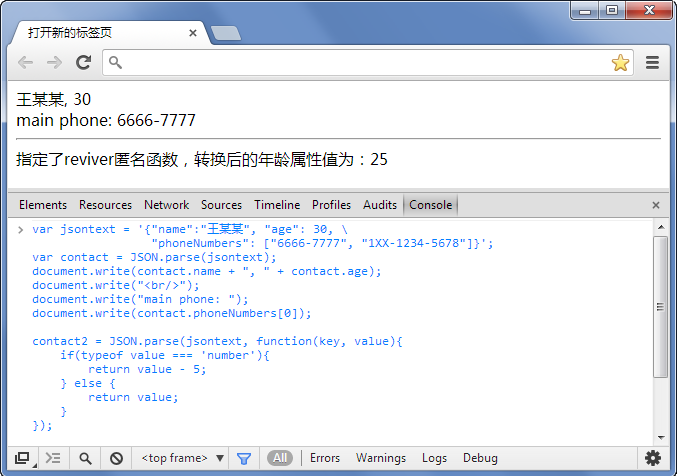
\includegraphics[width=0.9\textwidth]{figure/app-json.png}
\end{figure}
\end{easylist}
\end{frame}


\begin{frame}
\begin{center}
    \Huge END
\end{center}
\begin{figure}
    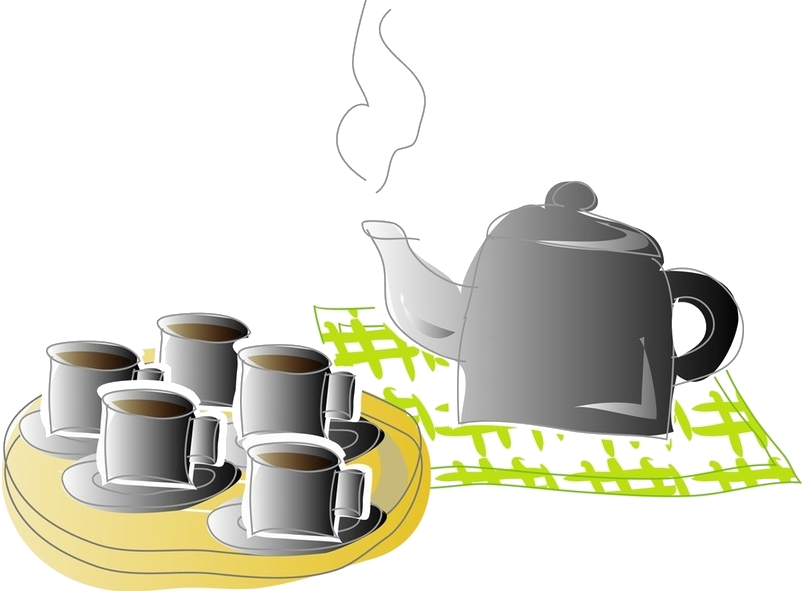
\includegraphics[width=0.75\textwidth]{figure/relax.png}
\end{figure}
\end{frame}
